\documentclass{article}
\usepackage[utf8]{inputenc}
\date{}
\usepackage{amsthm,amssymb,amsmath}
\usepackage{graphicx}
\graphicspath{ {./images/} }

\newtheorem*{theorem}{Theorem}

\newcommand{\NN}{\mathbb{N}}
\newcommand{\ZZ}{\mathbb{Z}}
\newcommand{\RR}{\mathbb{R}}
\newcommand{\QQ}{\mathbb{Q}}
\newcommand{\CC}{\mathbb{C}}


\title{ODE with Lipschitz Coefficients Draft}
\author{Phillip Yan} % Replace Me with your name!


\begin{document}

\maketitle

%%%%%%%%%%%%%%%%%%%%%%%%%%%%%%%%%%%%%%%%%%%%%%%%%%%%%%%%%%%%%%%%%%%%%%%%%%%%%%


\section{Introduction to ODEs}
To prove the existence and uniqueness of solutions to ODE's with Lipschitz coefficients, let us first introduce Ordinary Differential Equations. \\

\subsection{Solving ODEs and Examples}
\textbf{Definition: Ordinary Differential Equation:} A differential equation that is dependent on a single variable.

For this paper, we  will consider first-order ODE's as higher order ODE's can be turned into first-order ODE's as we will show later. An example of a first order ODE is:
$$\frac{dy}{dx} = f(x,y)$$
Intuitively, an ODE is a representation of a rate of change.
That is, the derivative of a function $\frac{dy}{dx}$ is expressed in terms of a function of $x$ and $y$ itself. 



A clear real world example can be seen in the expression of acceleration as the change in velocity. That is, 

$$\frac{dv}{dt} = a$$

where v is velocity, t is time, and a is acceleration per unit time. Here, instead of a function for velocity, we see the change of velocity expressed as a function of acceleration. \\

Because it no longer clearly provides a function to define the value of the dependent variable itself, one may wish to "solve" the ODE, or to find the unknown function(s) of $y=f(x)$ which satisfy the "description" of the ODE's rate of change. In the example above, it would be to determine the velocity function as based of the time variable t. \\

ODEs are often solved via an \textbf{initial value problem}. Given an ODE alongside an initial value $(x_0, y_0)$ such that $y(y_0) = x_0$, a solution can potentially be found. In the previous example, given a starting velocity at time 0, $y(0) = 5m/s$ alongside the ODE describing acceleration or the rate of change of velocity, intuitively it makes sense that one could determine velocity at any given point of time $t>0$. Mathematically, for simple ODE's one can simply integrating both sides of the ODE in a method called \textbf{direct integration}. In this case, we integrate with respect to t:

$$y = \int dy =  \int \frac{dy}{dt} dt = \int a dt = at + v_0$$
where $v_0$ is our starting velocity.

A more complex method of solving ODEs is \textbf{separation of variables}. Given an ODE which defines $y'$ in terms of both y and x values for some ODE:

$$ \frac{dy}{dx} = 10xy, y(0) = 1$$

we can solve this by isolating the two variables on either side of the equation. Refactoring the expression to

$$  \frac{dy}{y} = 10xdx$$
we can take the integral of both sides to solve the ODE:

$$ \int \frac{1}{y}dy = \int 10x dx $$
$$ \ln y  = 5x^2 + C$$
$$ y = e^{5x^2 + C}, C=0$$

\subsection{Existence}
Although there are many other methods to solve ODEs, as ODEs get more complex, the solution might not be immediately obvious. Sometimes they might not even exist. Thus, a key task is to determine under what conditions do solutions exist. An example of an ODE where the solution does not exist is 
$$ \frac{dy}{dx} = \frac{1}{x}, y(0) = 0$$

Note that this function $f(x,y)$ does not exist when $x = 0$, implying that the derivative of any potential solutions do not exist at that point. Indeed, when attempting to evaluate via direct integration we see:
$$y = \log x +C$$
Attempting finding a specific function with $y(0) = 0$ results in an undefined value for $\log x$, meaning that there does not exist any continuously differential function y such that y satisfies the ODE and the initial condition 

\subsection{Uniqueness}
At the same time, it is important to determine whether solutions are unique given a specific initial condition. Returning again to our velocity and acceleration example, we wouldn't want two different velocity functions for the ODE and initial value problem. (You might end up with two different velocity values at a given time with the exact same acceleration and starting velocity!)

An example of an ODE where the solution is not unique is

$$\frac{dy}{dx} = \sqrt{\|y\|}, y(0) = 0$$



Because of the absolute value, we must consider two cases, where $y>0$ and where $y<0$
Case 1 $(y>0)$:
Evaluating this ODE via separation of variables and then direct integration, we see
$$ y^{-\frac{1}{2}}\frac{dy}{dx} = 1$$
$$ \int y^{-\frac{1}{2}}dy = \int dx$$
$$ 2y^{\frac{1}{2}} = x$$
Thus, a solution is $y = \frac{(x+c)^2}{4}$

Case 2 $(y<0)$:
Following the same process, except for $-y$, we get:
$$ 2(-y^{\frac{1}{2}}) = x$$
Thus another solution is $y = -\frac{(x+c)^2}{4}$


Furthermore, note that the tautological function $y = 0$ also is a solution. With 3 solutions, we have the opposite problem as the previous ODE which had no solutions. Our paper seeks to address the conditions that need to be satisfied so that there is exactly 1 solution.

\subsection{Example ODE With One Unique Solution}
Consider the ODE:
$$\frac{dy}{dx} = y^2 + xy + x^2, y(0) = 0$$

As a slightly more complex differential equation, it is less immediately obvious whether a solution exists and if that solution is unique. One can't easily separate the variables and directly integrate. Thus, for differential equations like these, we need some general theorem to assert that a solution exists and is unique.

In fact, this is a solvable ODE with one unique solution. We'll show why later on in our discussion.


\subsection{Graphical Intuition}
Graphical intuition on the xy-plane might be helpful for our following discussion. Instead of a traditional graph of a function $y = f(x) = x$ which maps values of x to values of y, we consider a slope field on the xy-plane. At every point $x,y$, the slope $\frac{dy}{dx}$ is calculated as a function of x and y and plotted on the graph to produce a field of different "slopes" at all points in the graph. 

\begin{center}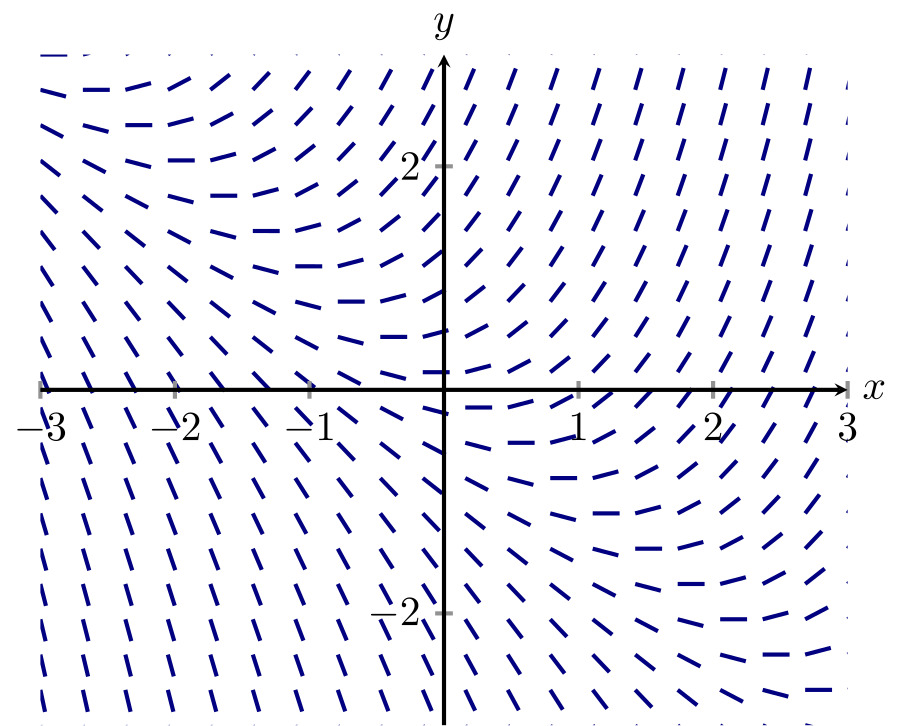
\includegraphics[width=7cm]{SlopeFieldMath.jpg} \\ A slope field for the ODE $\frac{dy}{dx} = y + x$\end{center}


Intuitively, when considering an initial value problem, one can potentially consider the initial coordinate pair given to be the coordinate of a boat, and the slope at any given point a current. Moving in the direction of the current, the "boat" traces out a curve which is the function that is the solution if it exists to the ODE.

\textbf{(I took some creative liberties in going over my intuition here, not sure if this intuition is sound; I'm also not sure if this is appropriate to include in a math paper)}

This intuition can help to serve as the basis to understand our approach in the following sections, especially Picard Iteration



\section{Lipschitz Continuity}
In this paper, we will prove that such solutions exist locally and are locally unique given that the ODE is Lipschitz continuous on a specified set.

Our first step in understanding when solutions exist and are unique in ODE's is to introduce a stronger form of continuity than our previous epsilon-delta definition of general continuity.

We first introduce the concept of \textbf{metric spaces}, of which $\mathbb{R}$ is an example which we have used in class. \\

\textbf{Definition: Metric Space} A metric space $(X, d_X)$ is a set $(X)$ with a notion of distance $(d_X)$ between its elements. 

In $\mathbb{R}^n$, this notion of distance is the 2-norm.

We now can now define Lipschitz continuity \\ 

\textbf{Definition: Lipschitz continuous} Given two metric spaces $(X, d_X)$ and $(Y, x_Y)$, a function $f: X \to Y$ is considered \textbf{Lipschitz continuous} if there exists $K \in \mathbb{R}$ such that for all $x_1, x_2 \in X$,
$$d_Y(f(x_1)-f(x_2)) \leq Kd_X(x_1-x_2)$$

Intuitively, a function is Lipschitz continuous over a certain interval if there exists a set constant value K that bounds the magnitude of the derivative at any point within the interval. Visually, at every point there exists a "double triangle" made from the two lines $y = K$ and $y = -K$ such that  the graph remains outside the triangle.\\

To see the relationship between this type of continuity and our more familiar epsilon-delta definition, we know that\\

\textbf{Proposition 1: }If a function is Lipschitz continuous over domain D, then it is also absolutely continuous over D\\


\textbf{Proof:} We will use an epsilon-delta proof. Because the function is Lipschitz, we know that for all values $x_1, x_2$ on this domain there exists a K such that $d_Y(f(x_1)-f(x_2)) \leq Kd_X(x_1-x_2)$. Given an arbitrary point $x_0 \in D$ and arbitrary $\epsilon >0$, we set our $\delta = \frac{\epsilon}{K}$. Thus, any value $x$ in the domain such that $d_X(x_1-x_2)<\delta$ means also that $d_X(x_1-x_2)<\frac{\epsilon}{K} \implies Kd_X(x_1-x_2)<\epsilon$. By definition of Lipschitz continuity, $d_Y(f(x_1)-f(x_2)) \leq Kd_X(x_1-x_2)$, so $d_Y(f(x_1)-f(x_2)) \leq Kd_X(x_1-x_2) < \epsilon \implies d_Y(f(x_1)-f(x_2))< \epsilon$
QED\\

At the same time Lipschitz continuity is actually stricter that general continuity since it bounds the derivative. \\

\textbf{Proposition 2:} Lipschitz continuity a subset of normal continuity \\

We can see this through example functions such as $e^x$ on $\mathbb{R}$ or $\sqrt{\|x\|}$ on $[-1,1] \in \mathbb{R}$ where although the function might be uniformly continuous, the derivative is unbounded on the given domain. For example, for $e^x$ there does not exist a constant K such that $\frac{d_Y(f(x_1)-f(x_2))}{d_X(x_1 - x_2)} \leq K$ where $x_1 = 0$ and as $x_2 \to \infty$ since $f(x_2)$ increases at a rate without bound. \\

\textbf{Not sure if I would need a formal proof above, I just assumed that I could just give an example since i already proved in Prop 1 that all functions that a Lipschitz continuous are also uniformly continuous. Is it good form to always prove all your propositions?} \\

The key idea here and across Lipschitz continuity as a whole is the importance of the coefficient $K$ and the importance of satisfying such a requirement in order to be considered Lipschitz continuous. The particular case when $K < 1$ also has special significance. \\

\textbf{Definition: Number} A \textbf{Contraction map} is defined on a metric space $(X, d_X)$ as a function $f: X \to X$ where there exists a real number $k$ such that for all $x_1, x_2$

$$d_Y(f(x_1)-f(x_2)) \leq kd_X(x_1-x_2)$$

A contraction map is therefore an example of a function that is Lipschitz continuous (and therefore uniformly continuous, as shown in Proposition 2) which satisfies a special case of Lipschitz continuity. The smallest value k that satisfies this expression can therefore be seen as the Lipschitz coefficient for the function. \\

Intuitively, because the distance between $f(x_1), f(x_2)$ is smaller than the initial distance, one can consider that applying this map multiple times (since it maps from a domain to itself) would cause the distance continuously "contract" after each iteration. Eventually, it would make sense for the points to potentially converge to a single point. Consider 
$$f(x) = x^2, x \in (-1,1) \in \mathbb{R}$$

This function is Lipschitz continuous on that given domain as there clearly exists some value K (say, K=10, or 100, or 1000 etc for clarity) that bounds the derivative. At the same time, the given domain of values $|x| < 1$ implies that $x^2 < |x|$. Eventually, one could intuit that the function might converge to 0. \\

We shall prove this idea of convergence in the following generalized Banach Fixed Point Theorem in the next section\\ 

\section{Banach Fixed Point Theorem}

Although in class we proved a version of the Banach Fixed Point Theorem, it required an assumption of a compact metric space. Here instead we shall prove a theorem with only the assumption of a complete metric space. \\

\textbf{Definition: Number} A \textbf{complete} metric space $(X, d_X)$ is defined as metric space where all Cauchy sequences of points in $X$ converges to a limit also in $X$. \\

Now we can express the Banach Fixed Point Theorem.\\

\textbf{Theorem 1: (Banach's Fixed Point Theorem)} Given a complete metric space $(X, d_X)$ and a contraction mapping on X $T: X \to X$, there exists some unique fixed point $x \in X$ such that $T(x) = x$. \\

\textbf{Proof of Theorem:} \\
We shall approach this proof in three steps. \\
\textbf{Part 1: }First, we will prove that such a sequence defined by the contraction mapping

$$x_0 = x_0, x_1 = T(x_0), x_2 = T(x_1), ... x_n = T(x_{n-1})$$

for some arbitrary initial value $x_0$ is Cauchy. 
Let us now find a relationship between the distance between any two adjacent elements in a sequence with the distance between the first two points. By definition of the above map, we can define the distance between two adjacent elements $x_{n+1}, x_{n}$ as
$$d(x_{n+1} , x_{n}) = d(T(x_{n+1}) , T(x_{n}))$$

By the definition of a contraction map, we know that there exists some K such that

$$d(T(x_{n}) , T(x_{n-1})) \leq Kd(x_{n+1}, x_{n}) $$

Repeating these past few steps, we see that:

$$d(x_{n+1} , x_{n}) \leq Kd(x_{n}, x_{n-1}) \leq K^2d(x_{n-1}, x_{n-2}) \leq ... \leq  K^{n}(x_{1}, x_{0}) $$
Inductively, therefore we can use the relationship:

$$d(x_{n+1} , x_{n}) \leq K^{n}(x_{1}, x_{0}) $$

Because all distance values are by definition positive and we know K to be between 0 and 1, we can use the fact that for any $m \geq n$

$$d(x_{n} , x_{m}) \leq d(x_n, x_{n+1}) + d(x_{n+1}, x_{n+2}) + d(x_{n+2}, x_{n+3}) +  ... + d(x_{m-1}, x_{m})$$

and then substitute the values for each of the distance measurements and say

$$ \leq (K^n + K^{n+1} + ... + K^{m-1})d(x_1, x_0) = K^n(1+ K + K^2 + ... + K^(m-n-1))(x_1, x_0)$$

which is less than the geometric series which is defined
$$ < K^n(1+ K + K^2 + ... )(x_1, x_0) \leq \frac{K^n}{1-K}(x_1, x_0)$$

Because the limit of $\frac{K^n}{1-K}$ as K approaches infinity is 0, we can see that for all $\epsilon$ a sufficiently large n means that all values $n_0$ greater than n result in 

$$\frac{K^{n_0}}{1-K}(x_1, x_0) \leq \epsilon$$

Thus, we have shown that this sequence is Cauchy. At the same time, because the metric space is defined as a complete metric space, we know that all Cauchy sequences converge. Thus, there exists some point $x_{\alpha}$ in $X$ such that this sequence (let's call it $x_n$) converges to $x_{\alpha}$, or $$x_n \to x_{\alpha}$$

\textbf{Part 2:} We now prove that this limit is indeed a fixed point
Returning to the fact $x_{n} = T(x_{n-1})$, we have already shown that when taking the limit of $x_{n}$ as n approaches infinity, we obtain $\lim_{n \to \infty} = x_{\alpha}$ for some value x that the sequence $x_n$ converges to. Thus,

$$x_{\alpha} = \lim_{n \to \infty} T(x_{n-1}) $$

Since T is Lipschitz continuous because it is a contraction map, we know from Proposition 1 that T is also continuous. Therefore, we can move the limit into the function to obtain:


$$ T(\lim_{n \to \infty}(x_{n-1})) = T(x_{\alpha}) $$

Thus, we have shown that $x_\alpha = T(x_\alpha)$ \\

\textbf{Part 3:} Our last step is to show that such a fixed point is unique. We will prove this with a proof by contradiction. Assume that there exists another distinct fixed point $y_{\alpha} \in X$. Then, $y_{\alpha} = T(y_{\alpha})$.

We know that the distance between the image of each point is strictly less than the distance between the two fixed points. That is,

$$d(T(x_{\alpha}), T(y_{\alpha})) \leq Kd(x_{\alpha}, y_{\alpha})$$



However, given the definition of fixed points, this also means

$$d(x_{\alpha}, y_{\alpha}) \leq Kd(x_{\alpha}, y_{\alpha})$$
which is impossible as with K  strictly less than 1, $d(x_{\alpha}, y_{\alpha})$ should instead be greater than $Kd(x_{\alpha}, y_{\alpha})$. Thus, the two distinct points do not exist, and $d(x_{\alpha}, y_{\alpha})$ is necessarily 0.

In these three steps, we have shown that such a unique point exists given a contraction mapping on a metric space \\
QED \\

This proof directly results in a useful Corollary.  \\
\textbf{Corollary:} The method to find a fixed point using Banach's Fixed Point Theorem is to apply the contraction mapping iteratively. \\

This will serve as an abstract basis for understanding Picard Iteration.

\section{Picard-Lindelöf Theorem}
Here we will finally integrate our discussion regarding Lipschitz Continuity and the Banach Fixed Point Theorem to produce a general theorem which dictates the conditions required for an ODE to have a locally existing solution that is also locally unique.

\subsection{Existence} 
\textbf{Theorem: }If a function f is continuous in an open rectangle
$$R = \{(x,y)| x_0-a<x<x_0+a \text{ and } y_0-b<y<y_0+b\}, (x_0, y_0) \in R$$
Then the initial value problem 

$$\frac{dy}{dx} = f(x,y), y(x_0) = y_0$$
has at least one solution within some sub-interval of $(a,b)$.



\subsection{Uniqueness} 

\textbf{Theorem: }If a function f and its partial derivative with respect to y $f_y$ are continuous in an open rectangle
$$R = \{(x,y)| x_0-a<x<x_0+a \text{ and } y_0-b<y<y_0+b\}, (x_0, y_0) \in R$$
Then the initial value problem 

$$\frac{dy}{dx} = f(x,y), y(x_0) = y_0$$

has a unique solution on some open sub-interval of (a,b).










\subsection{Proof}

Given such an initial value problem, we know that we can rewrite

$$\frac{dy}{dx} = f(x,y), y(x_0) = y_0$$

by integrating both sides in order to obtain:

$$ y(x) = x_0 + \int_{x_0}^{x}f(t,y(t))dt$$


We know that the given rectangle R is a metric space as it is a subset of $\mathbb{R}^2$ which is a metric space. 

Within this bounded metric space, we know that there exists a value M such that: 

$$M = |lub \{f(x,y) | (x,y) \in R\}|$$
In other words, M is colloquially the magnitude of the maximum of the slopes of the function within those bounds.

In order to use Banach's Fixed Point Theorem, we must also define a map T such that:

$$ T: R \to R$$
which we will set to be equal to our integrated ODE.

$$ T(y(x)) =  x_0 + \int_{x_0}^{x}f(t,y(t))dt$$

Note that this maps a function of y to another function of y within the defined rectangle metric space, which means that it maps the space of functions of y to itself.

We will now prove that this map is a contraction so we can finally use Banach's Fixed Point Theorem:

Consider two elements and apply the map T
$$T(y_1(x)) =  x_0 + \int_{x_0}^{x}f(t,y_1(t))dt$$
and
$$T(y_2(x)) =  x_0 + \int_{x_0}^{x}f(t,y_2(t))dt$$

Subtracting the equations from one another, we obtain:

$$T(y_1(x))- T(y_2(x)) = \int_{x_0}^{x}f(t,y_1(t))dt - \int_{x_0}^{x}f(t,y_2(t))dt$$
as the constant value $x_0$ disappears

Applying the absolute value to both sides to obtain a notion of distance in $\mathbb{R}^2$, we obtain:

$$|T(y_1(x))- T(y_2(x))| = |\int_{x_0}^{x}f(t,y_1(t))dt - \int_{x_0}^{x}f(t,y_2(t))dt|  = |\int_{x_0}^{x}f(t,y_1(t)) - f(t,y_2(t))dt|$$

Note that by moving the absolute value inside of the integral causes the resulting integral to be greater than or equal to the original as it instead considers the positive distance between the functions f.

$$ \leq \int_{x_0}^{x}|f(t,y_1(t)) - f(t,y_2(t))|dt$$
Since we are given that $f(x,y)$ is Lipschitz continuous with regards to y, we can express the difference between $f(x,y_1)$ and $f(x,y_2)$ as an inequality with respect to the product of a constant K and the difference between $y_1$ and $y_2$. That is,

$$ \leq \int_{x_0}^{x}K|y_1(t) - y_2(t)|dt = K\int_{x_0}^{x}|y_1(t) - y_2(t)|dt$$

Evaluating the integral while keeping in mind the bounds of the rectangle in terms of x ($x_0-a<x<x_0a$), we obtain

$$|T(y_1(x))-T(y_2(x))|  \leq Ka|y_1(t) - y_2(t)|$$

Note that although K, the Lipschitz constant that describes Lipschitz continuity in y for f might be fixed, by changing the value of the bounds for x on which we analyze whether or not T is a contraction, we can change the value of a. Thus, there exists a subset $[x_0-\epsilon, x+\epsilon]$ of of the bound $[x_0-a, x_0+a]$ such that $\epsilon K < 1 \implies |y_1(t) - y_2(t)| \text{has coefficient less than 1}$

Now that we have established that this is a contraction, we can use the Banach Fixed Point Theorem. The application of the theorem to this specific process is called \textbf{Picard Iteration}

$$y_1 = T(y_0) = y_0 + \int_0^t f(x, y_0)dt$$
$$y_2 = T(y_1) = y_0 + \int_0^t f(x, y_1)dt$$
$$...$$
We know that this process ultimately results in a unique fixed "function" by the Banach Fixed Point Theorem. That is, $\exists n$ such that 
$$y_n = T(y_n-1) = y_0 + \int_0^t f(x, y_0)dt = y_{n-1}$$

At this function $y_n$, we can see when we reintegrate that

$$\frac{dy_n}{dx} = f(x, y_n)$$
Furthermore, the previously integrated form shows that such a function $y_n$ also satisfies our initial value condition, $y(x_0) = y_0$
This is precisely the ODE we initially sought to solve.

Thus, $y_n$ is the unique solution to this ODE

QED

\subsection{Weakness} Note that the uniqueness and existence based on this proof of the Picard-Lindelöf Theorem only holds locally over a fixed interval. This could potentially be partially augmented by the \textbf{Cauchy-Peano Existence Theorem}, which, although only proves the existence of solutions, requires the ODE to only be generally continuous. This makes it much easier upon inspection to determine whether an ODE has solutions. However, the Cauchy-Peano Existence Theorem does not prove uniquness like the Picard-Lindelöf Theorem does.


\textbf{I didn't get a chance to implement the proof for the Cauchy-Peano Theorem but I'm planning on including it in the final draft to add a bit more of depth hopefully}

\section{Applications}
A potential real-world application can be seen in modeling species population over time. Since oftentimes our knowledge of a species' biomass is limited to their growth rate, ODEs are helpful in attempts to understand future population levels and potentially model the impact of different events. Given an initial population and a function detailing their growth, scientists are able to determine the biomass of a species

A popular and classical model in this regard is the \textbf{Lotka-Volterra} models.

\textbf{Not sure how much detail I should go into these example models, like should I include the differential equations and explain how it works?}

The Picard-Lindelöf Theorem is relevant here as if the requirements are satisfied, then exists a unique solution to an ODE over a certain local time interval. That is, given a growth rate, one can determine a unique function which represents total species population at any given period of time. The uniqueness aspect of the Theorem also guarantees that there aren't potentially multiple functions of population; there isn't a chance that one might obtain two different population values given the exact same starting conditions and differential equations.

\section{References}
Hirsch and Smale, ‘Differential equations, dynamical systems, and linear algebra’ \\ 
Arnold, Ordinary Differential Equations \\ 
https://www.ias.ac.in/article/fulltext/reso/022/05/0491-0507 \\ 
https://wiki.math.ntnu.no/\_media/tma4145/2020h/banach.pdf \\ 
https://ptolemy.berkeley.edu/projects/embedded/eecsx44/lectures/Spring2013/Picard.pdf\\












\end{document}
